\chapter{Implementation} \label{chap:4}

This chapter explain the steps taken to implement the research design and how it is addressed the issues occurred during implementation. Implementation can be divided as following sub topics.

\begin{itemize}
	\item Implementing server architectures in Ballerina
	\item Implementing test cases for performance evaluation
	\item Designing automated pipeline to obtain results
	\item Creating Machine learning models to classify programs
\end{itemize}

\section{Implementing server architectures in Ballerina}

Ballerina source code written Java and Ballerina itself.

This involves deeper analysis existing Ballerina run time. Ballerina has three main non-blocking thread pools. One thread pool (Worker thread) lies in the scheduler. Other two thread pools lies in the Netty layer. Ballerina's internal architecture is explained in-detail in chapter 3. Initial step is making Netty thread pool to have blocking IO.
The Netty layer integrated as separate library (trasport-http)\cite{transport-http}. Following code fragment shows the implemented changes.  \textit{workerGroup = new OioEventLoopGroup(200000);} specify the use of blocking thread in the tread pool and allowing up to 20,000 threads in the thread pool. This thread pool hand over the client workload to Ballerina Scheduler. This class is referred in the Ballerina run-time.

\begin{lstlisting}[language=Java]

	public class DefaultHttpWsConnectorFactory implements HttpWsConnectorFactory {
	
	private final EventLoopGroup bossGroup;
	private final EventLoopGroup workerGroup;
	private final EventLoopGroup clientGroup;
	private EventExecutorGroup pipeliningGroup;
	
	private final ChannelGroup allChannels = new DefaultChannelGroup(GlobalEventExecutor.INSTANCE);
	
	public DefaultHttpWsConnectorFactory(int serverSocketThreads, int childSocketThreads, int clientThreads) {
	bossGroup = new OioEventLoopGroup(4);
	workerGroup = new OioEventLoopGroup(200000);
	clientGroup = new NioEventLoopGroup(clientThreads);
	}
	
	...
\end{lstlisting}


The next architectural change is \textbf{remove Ballerina scheduler} and use only Netty threads to complete client request. Then the Ballerina scheduler is not involved in executing client request. Normal procedure is incoming request is handed over to scheduler thread pool. Then scheduler thread pool complete the execution using it's own threads and again handed over to Netty layer to send the client response. 

This implementation should be carried out carefully. If the implementation is erroneous or having bugs, it would produce wrong results. Thus extensive debugging was used while implementation .This was difficult due to tight coupling of Netty layer and Ballerina scheduler. In order to implement that I created separate \textbf{Task Executor} as \textit{MyExecutor}. Execution of client request is defined in that class. The \textit{submit()} method accept the incoming request and execute the instructions using incoming thread which is proceeded from Netty thread pool.


\begin{lstlisting}[language=Java]

public class BallerinaHTTPConnectorListener implements HttpConnectorListener {
...

@Override
public void onMessage(HttpCarbonMessage inboundMessage) {

...

MyExecutor.submit( service, httpResource.getName(), callback, properties, signatureParams);

...

\end{lstlisting}


Addition to major architectural changes, fine tuning to implemented architecture and existing architecture is carried out continuously. Those fine tunes assisted to narrow down to research to thread pool optimization. In the final phase existing Ballerina architecture is selected and tested with different thread pool numbers. Number of threads in the thread pool is set through environment variable. Following code snippet shows that.


\begin{lstlisting}[language=Java]
public class Scheduler {
 ...

// Setting Ballerina thread pool size 
private static String poolSizeConf = System.getenv(BLangConstants.BALLERINA_MAX_POOL_SIZE_ENV_VAR);

...

public Scheduler(boolean immortal) {
	try {
 		if (poolSizeConf != null) {
  			poolSize = Integer.parseInt(poolSizeConf);
 		}
	} catch (Throwable t) {
	
		// Log and continue with default
		err.println("ballerina: error occurred in scheduler while reading system variable:" +
		BLangConstants.BALLERINA_MAX_POOL_SIZE_ENV_VAR + ", " + t.getMessage());
	}
	this.numThreads = poolSize;
	this.immortal = immortal;

	console.println("Pool size: "+poolSize);
}

\end{lstlisting}



\section{Implementing test cases for performance evaluation}

Test cases were implemented in Ballerina language. This implementation is very crucial since all the results is depend on the designing of test programs. In the initial phases  all the test programs are designed to have IO calls and CPU intensive instructions. Some of test cases were designed by Ballerina team \cite{Ballerina_Performance} which was originally designed to evaluate performance of Ballerina run time. Those tests included external service calls (http requests). This research able to re-use them and reproduce the results.

Since Ballerina is service oriented language implementation is well structured. In Ballerina a service is packed to single unit. Following example represent the service called \textit{myservice}. That service is exposed outside via port number 9090. All the relevant implementation to this service goes inside the braces. There can be multiple services exposed via different ports. Structure of this is well suited with micro-service architecture.

\begin{lstlisting}[language=Java]
 service myservice on new http:Listener(9090) {
	
	}

\end{lstlisting}

Inside a service it can be implemented resource function. Single resource function can be considered as single endpoint in RESTful API. Following resource function represent the endpoint \textit{http://hostname:9090/book/someBookId}

\begin{lstlisting}[language=Java]

service myservice on new http:Listener(9090) {


@http:ResourceConfig {
methods: ["GET"], path: "/book/{bookId}"
}
resource function getById(http:Caller caller, http:Request req, string bookId) {
	json? payload = booksMap[bookId];
	http:Response response = new;
	if (payload == null) {
		response.statusCode = 404;
		payload = "Item Not Found";
	}
	response.setJsonPayload(untaint payload);
	var result = caller->respond(response);
	if (result is error) {
	log:printError("Error sending response", err = result);
	}
}

\end{lstlisting}

Similar to above resource funcnion all the test cases are enclosed as resource functions. Then the test cases are invoked by http request. Following code segment shows one test case used for testing. It includes single blocking IO call ( Databse call). 

\begin{lstlisting} [language=Java]
resource function db_select(http:Caller caller, http:Request request) returns error? {
	http:Response response = new;
	var params = request.getQueryParams();
	var id = <string>params.get("id")[0];//<string>params.id
	var query = "SELECT * FROM emp where id = "+id;
	
	stream<record{}, error> resultStream = mysqlClient4->query(<@untainted>query);
	
	record {|record {} value;|}|error? result = resultStream.next();
	
	error? e = resultStream.close();
	
	response.setTextPayload(<@untainted> io:sprintf("%s", result));
	check caller->respond(response);
	
	}
\end{lstlisting}

100 of programs similar to above are implemented to evalute test cases.

\section{Designing automated pipeline to obtain results}

This section explains how the results were obtained and what are the actions taken into account to ensure the accuracy. 

Proper testing environment is very important since results may inaccurate without proper isolation. Testing environments are isolated with used Docker \cite{docker} containers. It minimizes the interference occurred by other processes. Also it limits the resource usage by specifying the upper bound. 

Performance metrics are obtained primarily by Jmeter \cite{jmeter}. In order to minimize the instrumentation errors results are validated with load testing tool called Tsung \cite{tsung}.

\begin{figure}[htbp]
  \begin{center}
    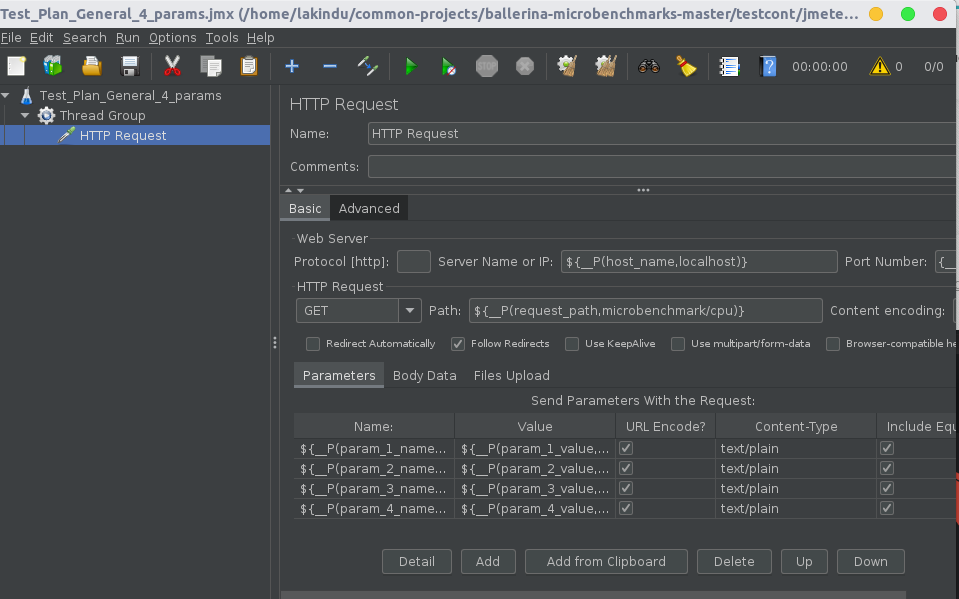
\includegraphics[scale=0.3]{figures/jmeter_sc.png}
    \end{center}
  \caption{Jmeter interface}
  \label{jmeter_ui}
\end{figure}


\begin{figure}[htbp]
	\begin{center}
		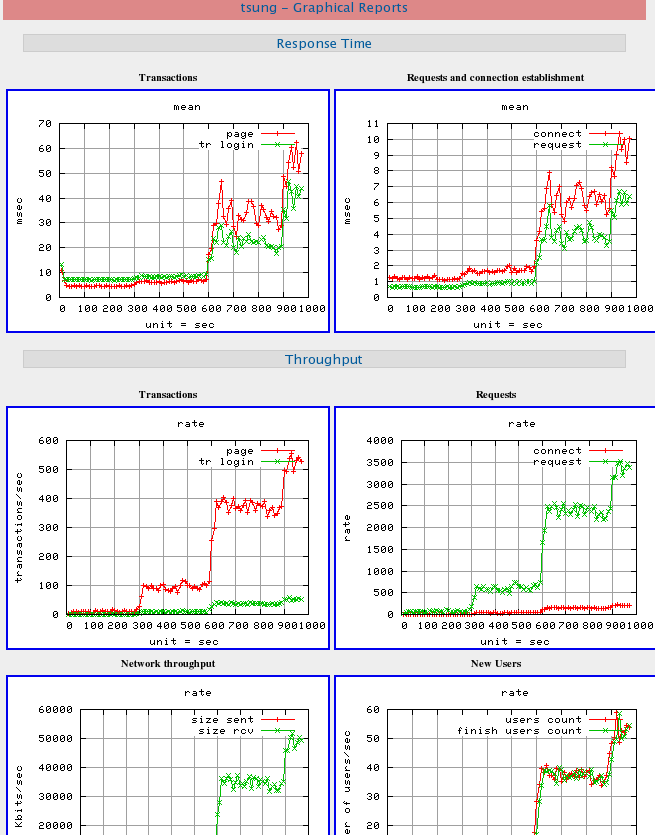
\includegraphics[scale=0.4]{figures/tsung-graph.png}
	\end{center}
	\caption{Tsung stat report}
	\label{tsung-graph}
\end{figure}


Jmeter have both command line and graphical user interface. Tsung configurations only available with command line and XML files. Configuring tests is easier in Jmeter than Tsung. Thus Tsung is only used to validate the results in early phases.  Several tests are executed using both tools and obtained the latency results to validate the tools. Some results are shown in table \ref{jmeter_and_tsung}. Average variance is \textit{0.29 ms}.

\begin{table}[htbp]
	\begin{center}
	\begin{tabular}{|l|l|l|l|}
		\hline
		Test   & Jmeter  & Tsung   & Description                                                                               \\ \hline
		test 1 & 27.42ms & 24.71ms & \begin{tabular}[c]{@{}l@{}}Database call - \\ concurrency level 80\end{tabular}           \\ \hline
		test 2 & 57.31ms & 57.22ms & \begin{tabular}[c]{@{}l@{}}External http call -\\ concurrency level 80\end{tabular}       \\ \hline
		test 3 & 44.97ms & 45.18ms & Merger sort - concurrency level 60                                                        \\ \hline
		test 4 & 34.76ms & 34.42ms & \begin{tabular}[c]{@{}l@{}}database call - \\ concurrency level 100\end{tabular}          \\ \hline
		test 5 & 28.44ms & 28.32ms & \begin{tabular}[c]{@{}l@{}}Prime number calculation -\\ concurrency level 80\end{tabular} \\ \hline
	\end{tabular}
	\end{center}
	\caption{Latency results comparison using Jmeter and Tsung}
	
	\label{jmeter_and_tsung}
\end{table}


Testing pipeline is consited of two parts, which are,

\begin{enumerate}
	\item Ballerina run time where tests were implemented
	\item Jmeter/Tsung clients to measure the performance metrics 
\end{enumerate}
	
Addition to above, database server, external HTTP server and grep server is designed to run tests. Figure \ref{testing_env} depict the architecture of testing environment. 3  \acrfull{VM} that are hosted in Google cloud is used. VM that running Ballerina run time and Jmeter client has 6 core CPU with 12 GB of memory. Other two VM are 2 core CPU with 4 GB of memory. In order to eliminate bottlenecks of external services CPU usage is monitored to keep the CPU usage under 80\%. Hence results are only depend on Ballerina run time. Since Ballerina run time, Jmeter client and Database server is hosted in same VM using docker Maximum CPU usage is limited to 2 cores for Jmeter and Ballerina run time. Database server is allocated with 1.2 CPU cores. With maximum concurrency level Database server use only 83\% CPU. 

Continuous monitoring ensured no bottleneck due to resource limitation. Testing pipeline is automated since duration of test is very long. Some tests were running for days and failing tests caused running them again. Implementation of pipeline is included in code listings.

\begin{figure}[htbp]
	\begin{center}
		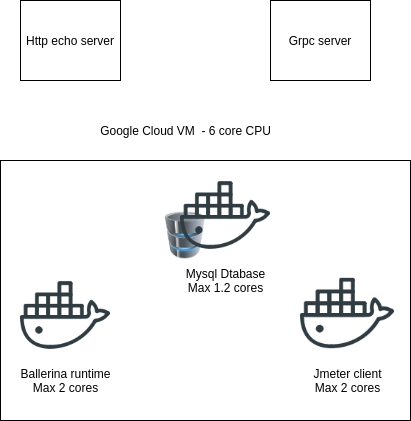
\includegraphics[scale=0.5]{figures/Tes_env.png}
	\end{center}
	\caption{Testing environment}
	\label{testing_env}
\end{figure}

\section{Creating Machine learning models to classify programs}

Final implementation of this research is build machine learning model to predict architecture based on programming features. Based on early results, the research is narrowed down to find the optimal thread pool size instead of predicting architecture. The final model predict the optimal thread pool size for the given program. Two approaches were used to obtain results. One is making the problem as classification problem and other is making it as regression problem. Then relevant metrics are compared to evaluate the best approach. Following machine learning models are used,

\begin{itemize}
	
	\item XGBoost
	\item Support Vector Machine
	\item Decision Tree
	\item Random Forest
	
\end{itemize}

Following code shows implementation of XGBoost regression model.

\begin{lstlisting} [language=Python]

from numpy import loadtxt
from xgboost import XGBRegressor
from sklearn.model_selection import train_test_split
from sklearn.metrics import accuracy_score
from sklearn.metrics import mean_absolute_percentage_error
from sklearn.metrics import mean_squared_error

def cross_validation_r(model,X,Y):

	cv = ShuffleSplit(n_splits=5, test_size=0.3, random_state=1)
	
	scores = cross_validate(model, X, Y, cv=cv , scoring=['neg_mean_squared_error','neg_mean_absolute_percentage_error'])
	
	
	cv_mape=scores['test_neg_mean_absolute_percentage_error']
	cv_mse=scores['test_neg_mean_squared_error']
	
	print("MAPEs: ",cv_mape)
	print("MSEs: ",cv_mse)
	
	print("MAPE: %0.2f%% with a standard deviation of %0.2f" % (abs(cv_mape.mean()*100), cv_mape.std()))
	print("MSE: %0.2f  with a standard deviation of %0.2f" % (abs(cv_mse.mean()), cv_mse.std()))
	
# load data
dataset = loadtxt('g_dataset_class_2.csv', delimiter=",")
# split data into X and y
X = dataset[:,0:5]
Y = dataset[:,6]
# split data into train and test sets
seed = 6
test_size = 0.3

X_train, X_test, y_train, y_test = train_test_split(X, Y, test_size=test_size, random_state=seed)
# fit model no training data
model = XGBRegressor()

model.fit(X_train, y_train)
# make predictions for test data
y_pred = model.predict(X_test)
predictions = [round(value) for value in y_pred]


# Cross validation
print("# cross validated evaluations")
print(cross_validation_r(model,X,Y))

# cross validated evaluations
MAPE: 7.92% with a standard deviation of 0.01
MSE: 1.46  with a standard deviation of 0.15

\end{lstlisting}

In order to tune hyper parameters of the machine learning model, following implementation is used. Then the machine learning model is retrained with optimal parameters rather than default parameters.

\begin{lstlisting} [language=Python]

def hyperparameter_tuning(tr_features, tr_labels):
	# Number of trees in random forest
	n_estimators = [int(x) for x in np.linspace(start = 200, stop = 2000, num = 1000)]
	# Number of features to consider at every split
	max_features = ['auto', 'sqrt']
	# Maximum number of levels in tree
	max_depth = [int(x) for x in np.linspace(5, 150, num = 50)]
	max_depth.append(None)
	# Minimum number of samples required to split a node
	min_samples_split = [x for x in range(1,51)]
	# Minimum number of samples required at each leaf node
	min_samples_leaf = [x for x in range(1,51)]
	# Method of selecting samples for training each tree
	bootstrap = [True, False]
	# Create the random grid
	random_grid = {
	'max_features': max_features,
	'max_depth': max_depth,
	'min_samples_split': min_samples_split,
	'min_samples_leaf': min_samples_leaf,
	}
	
	rf_hyper = tree.DecisionTreeRegressor()
	rf_random = model_selection.RandomizedSearchCV(estimator = rf_hyper, param_distributions = random_grid, n_iter = 100, cv = 3, verbose=2, random_state=42, n_jobs = -1)
	# Fit the random search model
	rf_random.fit(tr_features, tr_labels)
	return rf_random.best_params_
	
	a =hyperparameter_tuning(X_train,y_train)
	return a

\end{lstlisting}



